\documentclass[a4paper,12pt]{book}

\usepackage{ZeroSeven}

\titlepage{}

\author{Ludovico Brocca}
\date{26-11-2018}
\intestazioni{
\includegraphics[scale=0.3]{images/logo_intestazione}}
\pagestyle{myfront}
\begin{document}
\begin{titlepage}
	\centering
	{\huge\bfseries MegAlexa\par}
	Arricchitore di skill di Amazon Alexa
	\line(1,0){350} \\
	{\scshape\LARGE Analisi Dei Requisiti \par}
	\vspace{1cm}
	{\scshape Gruppo ZeroSeven \par}
	\logo
	%devono essere compilati questi campi ogni volta
	\begin{tabular}{c|c}
		{\hfill \textbf{Versione}} 			& 0.0.1				\\
		{\hfill\textbf{Data Redazione}} 	& 19-12-2018		\\ 
		{\hfill\textbf{Redazione}} 			&  		Ludovico Brocca			\\ 
		{\hfill\textbf{Verifica}} 				&  	Nome Cognome			\\ 
		{\hfill\textbf{Approvazione}} 		&  		Nome Cognome			\\ 
		{\hfill\textbf{Uso}} 					& 		Esterno		\\ 
		{\hfill\textbf{Distribuzione}} 			& 			Prof. Tullio Vardanega \\ & Prof. Riccardo Cardin \\ & Gruppo ZeroSeven		\\ 
		{\hfill\textbf{Email di contatto}} & zerosevenswe@gmail.com \\
	\end{tabular}
\end{titlepage}
	

	
	\label{LastFrontPage}
	\newpage	
	\begin{center}
	\textbf{Registro delle modifiche}
	\end{center}
	\begin{center}
		\begin{tabularx}{\textwidth}{|c|c|X|X|c|}
			\hline
			\textbf{Versione} & \textbf{Data} & \textbf{Descrizione} & \textbf{Autore} & \textbf{Ruolo} \\ 
			\hline
			3.0.0 & 2019-04-11 & Approvazione per il rilascio RQ & Ludovico Brocca & Responsabile \\
			\hline
			2.1.0 & 2019-04-09 & Verifica documento & Ludovico Brocca & Verificatore \\
			\hline
			2.0.6 & 2019-04-08 & Aggiunto riferimento metriche alla sezione \S\ref{MetricheObbiettivi} &Matteo depascale & Amministratore \\
			\hline 
			2.0.5 & 2019-04-08 & Modifica sezioni \S\ref{Verifica}  e \S\ref{Validazione} & Matteo depascale & Amministratore \\
			\hline
			2.0.4 & 2019-04-08 & Aggiunti comandi personalizzati alla sezione \S\ref{NormeRedazionali} &Matteo depascale & Amministratore \\
			\hline
			2.0.3 & 2019-04-04 & Aggiunta voci a \S\ref{ListaControllo} & Matteo depascale & Amministratore \\
			\hline
			2.0.2 & 2019-04-01 & Stesura sezioni \S\ref{DiagrammiDelleClassi}, \S\ref{DiagrammiPackage}, \S\ref{DiagrammiSequenza} e \S\ref{DiagrammiAttivita}  & Bianca Andreea Ciuche & Amministratore \\
			\hline
			2.0.1 & 2019-03-23 & Modifica \ref{Documentazione fornita} Corretti numeri di sezione & Bianca Andreea Ciuche & Amministratore \\
			\hline
			2.0.0 &2019-03-07 & Approvazione per il rilascio & Gian Marco Bratzu& Responsabile\\
			\hline
			1.2.0 &2019-03-02 & Verifica documento &Andrea Deidda& Verificatore\\
			\hline
			1.1.2 &2019-02-13 &Stesura \S\ref{calcoloOre} &Ludovico Brocca& Amministratore\\
			\hline
			1.1.1 &2019-02-13 &Modifica\S \ref{anDinamica} &Ludovico Brocca& Amministratore\\
			\hline
			1.1.0 &2019-02-07 &Verifica \S\ref{processo}, \ref{metriche}, \S\ref{progettazione} &Gian Marco Bratzu& Verificatore\\
			\hline
			1.0.4 &2019-02-04&Stesura \S\ref{processo}&Ludovico Brocca& Analista\\
			\hline
			1.0.3 & 2019-02-03 & Modifica \S\ref{metriche} & Stefano Zanatta & Amministratore\\
			\hline
			1.0.2 & 2019-02-02 & Stesura \S\ref{metriche} & Bianca Andreea Ciuche & Amministratore\\
			\hline
			1.0.1 & 2018-01-12 & Stesura \S\ref{progettazione} & Mirko Franco & Amministratore \\
			\hline
			1.0.0 & 2018-01-09 & Approvazione per il rilascio & Stefano Zanatta & Responsabile\\
			\hline
			0.2.0 & 2018-12-29 & Verifica documento & Stefano Zanatta & Verificatore\\
			\hline
			0.1.0 & 2018-12-18 & Verifica \S\ref{PdS} & Mirko Franco & Verificatore\\
			\hline
			0.0.6 & 2018-12-21 & Modifica \S\ref{Intro} & Andrea Deidda & Amministratore\\
			\hline
			0.0.5 & 2018-12-17 & Stesura \S\ref{Po} & Ludovico Brocca & Amministratore\\
			\hline
			0.0.4 & 2018-12-16 & Stesura \S\ref{Pp} & Matteo Depascale & Amministratore\\
			\hline
			0.0.3 & 2018-12-16 & Stesura \S\ref{Intro} & Bianca Ciuche & Amministratore\\
			\hline
			0.0.2 & 2018-12-10 & Stesura \S\ref{PdS} & Gian Marco Bratzu & Amministratore\\	
			\hline
			0.0.1 & 2018-12-08 & Struttura documento  & Ludovico Brocca & Amministratore\\
			\hline
	\end{tabularx}
	\end{center}

\newpage
	\pagestyle{mymain}
	\tableofcontents
	\chapter{Introduzione}
\label{introduzione}
\section{Scopo del documento}
Il \textit{Piano di Qualifica} ha lo scopo di definire gli obbiettivi di qualità che il gruppo perseguita per il proprio prodotto. Per ottenere tali obbiettivi è necessario un processo di verifica continua di ogni attività. Questo consente di rilevare e correggere le anomalie riscontrate tempestivamente.\\
Questo documento descrive nel dettaglio la qualità dei processi più vicini nel tempo e ad alto livello quelli più lontani, per poi essere aggiornato con nuovi contenuti ogni volta che il gruppo lo ritiene necessario.
\section{Scopo del prodotto}
Lo scopo del progetto è quello di sviluppare un applicativo Mobile in grado di creare delle routine personalizzate per gli utenti gestibili tramite\glossario{Alexa}di\glossario{Amazon}. L'obbiettivo è quello di creare\glossario{skill}in grado di avviare\glossario{workflow}creati dagli utenti fornendogli dei\glossario{connettori}.
\section{Glossario}
Al fine di evitare ogni ambiguità di linguaggio e massimizzare la comprensione dei documenti, i termini tecnici, di dominio, gli acronimi e le parole che necessitano di essere chiarite, sono riportate nel \textit{Glossario v1.0.0}.\\
Ogni occorrenza di vocaboli presenti nel \textit{Glossario} è marcata da una "G" maiuscola in pedice.
\section{Riferimenti}
\subsection{Normativi}
\begin{itemize}
	\item  \textbf{Norme di Progetto}: \textit{Norme di Progetto v1.0.0};
	\item \textbf{Capitolato$_{G}$ C4}:\glossario{MegAlexa}: arricchitore di skill di Amazon Alexa.
	\item \textbf{Ciclo di Deming}
	\footnote{\url{https://it.wikipedia.org/wiki/Ciclo_di_Deming}}
\end{itemize}
\subsection{Informativi}\label{rfinf}
\begin{itemize}
	\item \textbf{Piano di Progetto}: \textit{Piano di Progetto v1.0.0};
	\item \textbf{Complessità ciclomatica}
	\item \textbf{Software Testing Fundamentals: Methods and Metrics} di Marnie L. Hutcheson, Wiley Publishing, Inc.  
	\footnote{\url{https://www.math.unipd.it/~tullio/IS-1/2018/Progetto/C4.pdf}}.
	
	
\end{itemize}

	\chapter{Descrizione generale}

\section{Scopo del prodotto}
L'obbiettivo del prodotto è quello di permettere ad un utente di creare uno o più \glossario{workflow} personali leggibili tramite un dispositivo \glossario{Alexa}.
Per poter usufruire delle funzionalità di tale prodotto l'utente dovrà prima effettuare l'autenticazione all'applicativo con apposite username e password.
Il prodotto realizzato sarà multilingua, quindi potrà essere utilizzato da un numero più ampio di utenti.


\section{Funzioni del prodotto}
\begin{itemize}
	\item Permettere il login all'utente;
	\item Creare dei \glossario{workflow} personalizzabili;
	\item Pemettere la modifica e la cancellazione dei \glossario{workflow};
	\item Possiblità di eseguire i \glossario{workflow} tramite \glossario{Alexa}; 
	\item Ottenere un output vocale dal dispositivo \glossario{Alexa} in base al workflow eseguito;
\end{itemize}

\section{Caratteristiche degli utenti}
Il prodotto è sviluppato per i privati e le aziende che vogliono utilizzare l'assistente vocale \glossario{Alexa} di Amazon.
L'utente, per accedere al sistema, dovrà essere registrato con una propria mail e password e aver effettuato un \textit{account} \glossario{linking} con il proprio account Amazon personale.


\section{Vincoli di progettazione}
\subsection{Requisiti desiderabili}
\begin{itemize}
	\item Realizzare una mobile app per dispositivi Android;
	\item
	\item
	\item
\end{itemize}
\subsection{Requisiti opzionali}
\begin{itemize}
	\item Sviluppo del prodotto per dispositivi iOS;
	\item Sviluppo del prodotto con interfaccia web;
\end{itemize}
	\chapter{Casi d'uso}
In questa sezione sono elencati i casi d'uso del \textit{progetto$_{G}$}\glossario{MegAlexa}dedotti da un'attenta indagine ed analisi da parte dei membri del gruppo sugli attori principali del sistema, sulle loro caratteristiche e possibilità.
Ogni caso d'uso è identificato da un codice univoco e possiede una struttura interna accuratamente definita nel documento Norme Di Progetto 
v1.0.0.
\section{Attori dei casi d'uso}
\textbf{Attori primari}
\begin{itemize}
	\item \textbf{Utente non autenticato}: si riferisce all'utente del sistema che non ha ancora eseguito il login;
	\item \textbf{Utente autenticato}: si riferisce all'utente del sistema che ha effettuato il login ed è stato autenticato.
\end{itemize}
\textbf{Attori secondari}
\begin{itemize}
	\item \textbf{Amazon$_{G}$}.
\end{itemize}

\section{Caso d'uso UC1: Scenario principale dell'utente non autenticato}

\begin{figure}[h]
	\centering
	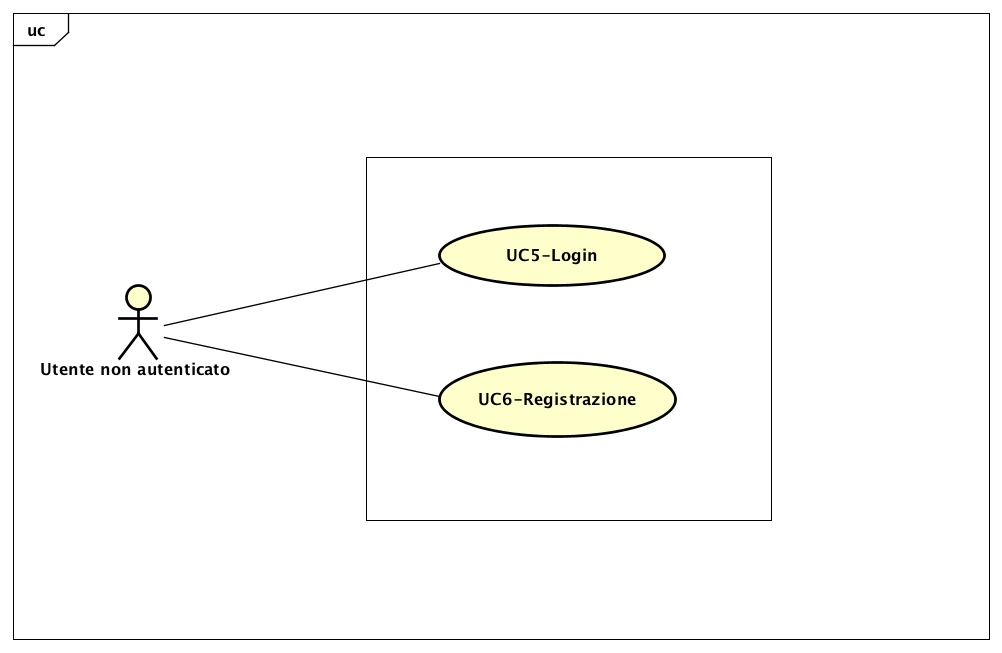
\includegraphics[scale=0.4]{Diagram/UC1.png}
	\caption{Scenario principale}\label{}
\end{figure}

\begin{itemize}
	\item \textbf{Attori primari}: Utente non autenticato;
	\item \textbf{Attori secondari}: Amazon;
	\item \textbf{Descrizione:} Un utente non autenticato può registrarsi al nostro servizio se non ha ancora un account o effettuare il login, nel caso fosse già registrato;
	\item \textbf{Precondizione:} L'applicazione è avviata e pronta all'uso;
	\item \textbf{Flusso principale degli eventi}:
	\begin{enumerate}
		\item L'utente ha la possibilità di: Registrazione (UC1.1);
		\item L'utente ha la possibilità di: Login (UC1.2).
	\end{enumerate}
	\item \textbf{Postcondizione}: L'applicazione ha ricevuto tutte le informazioni dell'utente non autenticato sulle operazioni che vuole eseguire.
\end{itemize}

\section{Caso d'uso UC1.1: Registrazione}
\begin{figure} [h]
	\centering
	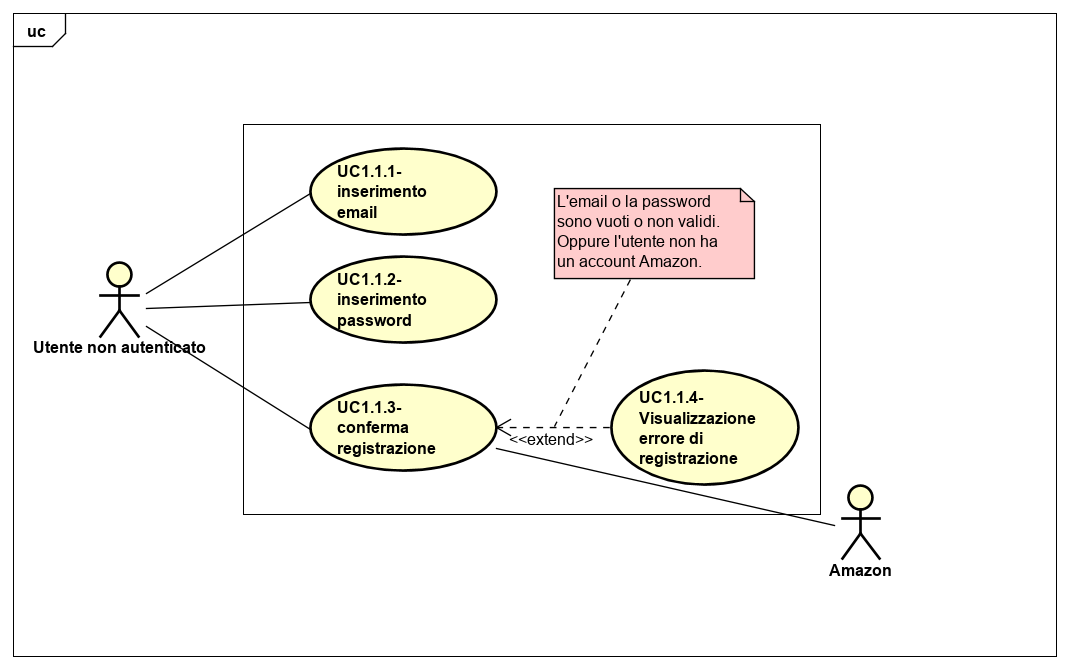
\includegraphics[scale=0.4]{./Diagram/UC1-1.png}
	\caption{Registrazione}\label{}
\end{figure}
\begin{itemize}
	\item \textbf{Attori primari}: Utente non autenticato;
	\item \textbf{Attori secondari}:\glossario{Amazon};
	\item \textbf{Descrizione}: Per accedere al sistema è necessario possedere un account;
	\item \textbf{Precondizione}: L'attore non possiede un account per accedere al sistema;
	\item \textbf{Flusso principale degli eventi}: 
	\begin{enumerate}
		\item L'attore inserisce la propria email (UC1.1.1);
		\item L'attore inserisce la propria password (UC1.1.2);
		\item L'attore conferma la registrazione(UC1.1.3).
	\end{enumerate}
	\item \textbf{Scenario alternativo}: L'attore dopo aver confermato le proprie credenziali visualizza un messaggio d'errore (UC1.1.4);
	\item \textbf{Postcondizione}:E' stato creato un account per accedere al sistema;
	\item \textbf{Estensioni}:
	\begin{enumerate}
		\item	Visualizzazione errore di registrazione(UC1.1.4).
	\end{enumerate}
\end{itemize}

\section{Caso d'uso UC1.1.1: Inserimento email}
\begin{itemize}
	\item \textbf{Attori primari}: Utente non autenticato;
	\item \textbf{Descrizione}: L'attore deve inserire la propria email per effettuare la  registrazione;
	\item \textbf{Precondizione}: Il sistema mostra il campo per l'inserimento della email;
	\item \textbf{Flusso principale degli eventi}: L'attore inserisce la propria email per effettuare la registrazione;
	\item \textbf{Postcondizione}: E' stata inserita l'email dell'attore nel campo opportuno.
\end{itemize}
\section{Caso d'uso UC1.1.2: Inserimento password}
\begin{itemize}
	\item \textbf{Attori primari}: Utente non autenticato;
	\item \textbf{Descrizione}: L'attore deve inserire la propria password per effettuare la registrazione;
	\item \textbf{Precondizione}: Il sistema mostra il campo per l'inserimento della password;
	\item \textbf{Flusso principale degli eventi}: L'attore inserisce la propria password per effettuare la registrazione;
	\item \textbf{Postcondizione}: È stata inserita la password dell'attore nel campo opportuno.
\end{itemize}

\section{Caso d'uso UC1.1.3: Conferma registrazione}
\begin{itemize}
	\item \textbf{Attori primari}: Utente non autenticato;
	\item \textbf{Descrizione}: L'attore dopo aver compilato i campi richiesti decide di confermare  la registrazione;
	\item \textbf{Precondizione}: Il sistema mostra un pulsante per confermare la registrazione;
	\item \textbf{Flusso principale degli eventi}:L'attore decide di confermare la registrazione per completarla;
	\item \textbf{Postcondizione:} Il sistema registra l'attore poiché questo ha confermato l'operazione;
	\item \textbf{Estensione:}
	\begin{itemize}
		\item Visualizzazione dell'errore di registrazione(UC1.1.4).
	\end{itemize}
\end{itemize}


\section{Caso d'uso UC1.1.4: Visualizzazione dell'errore di registrazione}
\begin{itemize}
	\item \textbf{Attori primari}: Utente non autenticato;
	\item \textbf{Descrizione}: L'attore visualizza un errore nel caso avesse compilato i campi con dati errati;
	\item \textbf{Precondizione}: Il sistema ha ricevuto campi dati errati: vuoti o non validi;
	\item \textbf{Flusso principale degli eventi}: L'attore visualizza il messaggio d'errore relativo al campo dato del:
	\begin{itemize}
		\item E-mail;
		\item Password.
	\end{itemize}
	\item \textbf{Postcondizione:} Il sistema mostra un messaggio d'errore per segnalare il tentativo di registrarsi con campi dati errati.
\end{itemize}

\section{Caso d'uso UC1.2: Login}
\begin{figure} [h]
	\centering
	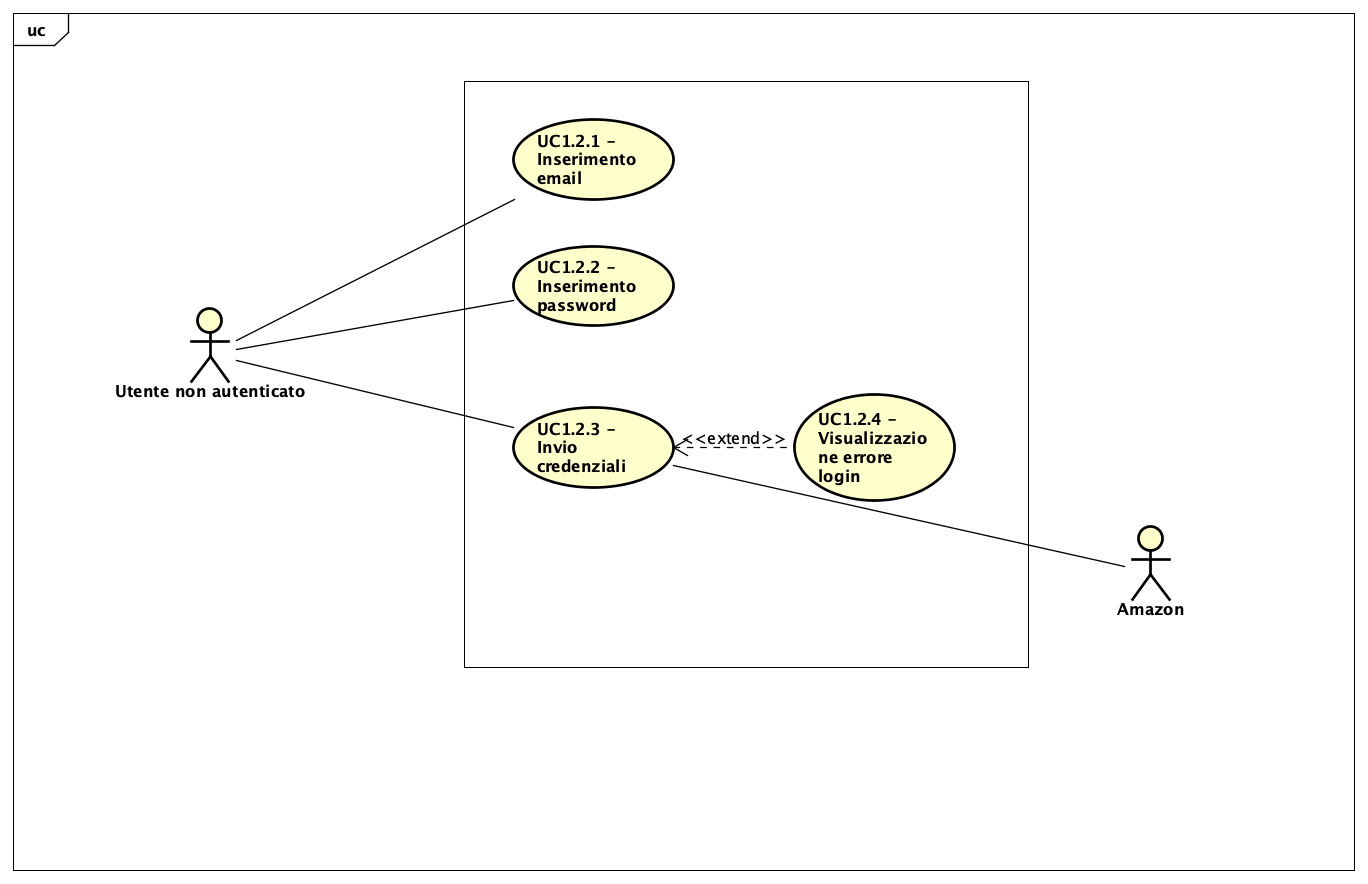
\includegraphics[scale=0.4]{./Diagram/UC1-2.png}
	\caption{Login}\label{}
\end{figure}
\begin{itemize}
	\item \textbf{Attori primari}: Utente non autenticato;
	\item \textbf{Attori secondari}:\glossario{Amazon};
	\item \textbf{Descrizione}: Il sistema è avviato, ma è necessario effettuare il login per accedervi;
	\item \textbf{Precondizione}: Il sistema non permette l'accesso all'utente non autenticato;
	\item \textbf{Flusso principale degli eventi}:
	\begin{enumerate}
		\item L'utente inserisce la propria email (UC1.2.1);
		\item L'utente inserisce la propria password (UC1.2.2);
		\item L'utente invia le credenziali (UC1.2.3).
	\end{enumerate}
	\item \textbf{Scenario alternativo}: L'utente dopo aver inviato le proprie credenziali visualizza un messaggio d'errore (UC1.2.4);
	\item \textbf{Postcondizione}: Il sistema permette l'accesso all'utente che ora diventa un utente autenticato; 
	\item \textbf{Generalizzazioni}:
	\begin{enumerate}
		\item Login automatico (UC1.3).
	\end{enumerate}
\end{itemize}


\section{Caso d'uso UC1.2.1: Inserimento email}
\begin{itemize}
	\item \textbf{Attori primari}: Utente non autenticato;
	\item \textbf{Descrizione}: L'utente inserisce la sua email per effettuare il login;
	\item \textbf{Precondizione}: Il sistema fa visualizzare il campo email;
	\item \textbf{Flusso principale degli eventi}: L'attore inserisce la sua mail per effettuare il login;
	\item \textbf{Postcondizione:} E' stata inserita la mail dell'attore nel campo predisposto. 
\end{itemize}

\section{Caso d'uso UC1.2.2: Inserimento password}
\begin{itemize}
	\item \textbf{Attori primari}: Utente non autenticato;
	\item \textbf{Descrizione}: L'utente inserisce la sua password per effettuare il login;
	\item \textbf{Precondizione}: Il sistema fa visualizzare il campo password;
	\item \textbf{Flusso principale degli eventi}: L'attore inserisce la sua password per effettuare il login;
	\item \textbf{Postcondizione:} E' stata inserita la password dell'attore nel campo predisposto. 
\end{itemize}
\section{Caso d'uso UC1.2.3: Invio credenziali}
\begin{itemize}
	\item \textbf{Attori primari}: Utente non autenticato;
	\item \textbf{Descrizione:} Dopo aver inserito tutti i dati l'utente conferma il login;
	\item \textbf{Precondizione}: Il sistema far visualizzare la pagina di login;
	\item \textbf{Flusso principale degli eventi}: L'attore dopo aver inserito le credenziali può confermare il login;
	\item \textbf{Postcondizione}: L'utente è riconosciuto dal sistema come utente autenticato;
	\item \textbf{Scenari alternativi}: L'utente inserisce credenziali errate e viene visualizzato un messaggio d'errore;
	\item \textbf{Estensioni}:
	\begin{enumerate}
		\item Visualizzazione errore login (UC1.2.4).
	\end{enumerate} 
\end{itemize}
\section{Caso d'uso UC1.2.4: Visualizzazione errore login}
\begin{itemize}
	\item \textbf{Attori primari}: Utente non autenticato;
	\item \textbf{Descrizione:} L'attore può aver inserito delle credenziali errate;
	\item \textbf{Precondizione}: Il sistema ha ricevuto campi dati errati;
	\item \textbf{Flusso principale degli eventi}: L'attore visualizza un messaggio d'errore;
	\item \textbf{Postcondizione:} L'utente non è riconosciuto dal sistema.
\end{itemize}
\section{Caso d'uso UC1.3: Login automatico}
\begin{itemize}
	\item \textbf{Attori primari}: Utente non autenticato;
	\item \textbf{Attori secondari}:\glossario{Amazon};
	\item \textbf{Descrizione}: Il sistema è avviato, ma è necessario effettuare il login per accedervi;
	\item \textbf{Precondizione}: Il sistema non permette l'accesso all'utente non autenticato;
	\item \textbf{Scenario alternativo}: L'utente dopo aver inviato le proprie credenziali visualizza un messaggio d'errore (UC1.2.4);
	\item \textbf{Postcondizione}: Il sistema permette l'accesso all'utente che ora diventa un utente autenticato.
\end{itemize}
\section{Caso d'uso UC2: Scenario principale dell'utente autenticato}
\begin{figure} [h]
	\centering
	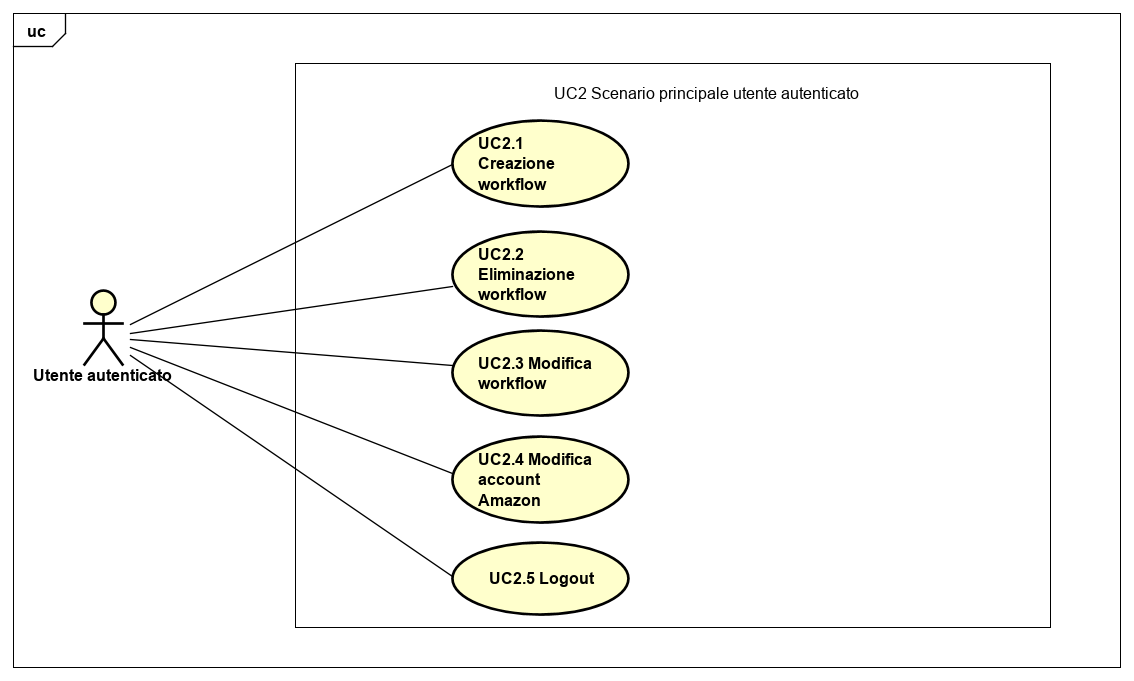
\includegraphics[scale=0.4]{./Diagram/UC2.png}
	\caption{Scenario principale dell'utente autenticato }\label{}
\end{figure}
\begin{itemize}
	\item \textbf{Attori primari}: Utente autenticato;
	\item \textbf{Descrizione:} L'attore può creare, modificare ed eliminare un\glossario{workflow}, modificare i propri dati personali ed eseguire il logout;
	\item \textbf{Precondizione:} Il sistema mostra la pagina principale per l'utente autenticato;
	\item \textbf{Flusso principale degli eventi:}
	\begin{enumerate}
		\item L'utente può creare un\glossario{workflow}(UC2.1);
		\item L'utente può eliminare un workflow (UC2.2);
		\item L'utente può modificare un workflow (UC2.3);
		\item L'utente può modificare l'account\glossario{Amazon}(UC2.4);
		\item L'utente può effettuare il Logout (UC2.5).
	\end{enumerate}
	\item \textbf{Postcondizione:} Il sistema ha ricevuto le informazioni riguardanti i comandi che l'utente vuole eseguire.
\end{itemize}
\section{Caso d'uso UC2.1: Creazione workflow}
\begin{figure} [h]
	\centering
	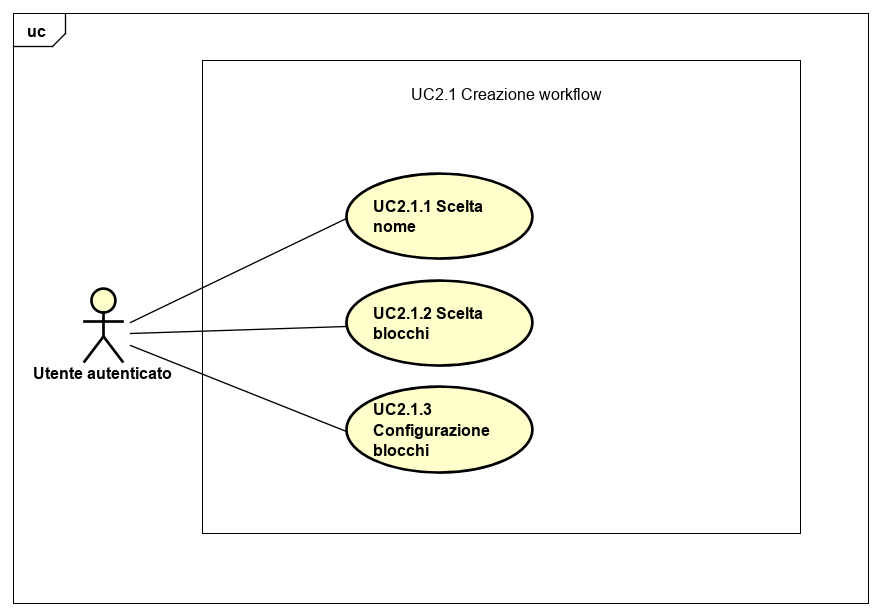
\includegraphics[scale=0.4]{./Diagram/UC2-1.png}
	\caption{Scenario principale dell'utente autenticato }\label{}
\end{figure}
\begin{itemize}
	\item \textbf{Attori primari}: Utente autenticato;
	\item \textbf{Descrizione:} L'attore può creare un\glossario{workflow}selezionando e configurando i blocchi disponibili;
	\item \textbf{Precondizione:} Il sistema mette a disposizione un form per la creazione di un \textit{workflow$_{G}$};
	\item \textbf{Flusso principale degli eventi:}
	\begin{enumerate}
		\item L'utente sceglie il nome del\glossario{workflow}(UC2.1.1);
		\item L'utente seleziona quali blocchi vuole usare (UC2.1.2);
		\item L'utente configura i blocchi selezionati (UC2.1.3).
	\end{enumerate}
	\item \textbf{Postcondizione:} Il sistema contiene il workflow desiderato dall'attore.
\end{itemize}
\section{Caso d'uso UC2.1.1: Scelta nome }
\begin{itemize}
	\item \textbf{Attori primari}: Utente autenticato;
	\item \textbf{Descrizione:} L'attore inserisce il nome del \textit{workflow$_{G}$};
	\item \textbf{Precondizione:} Il sistema mette a disposizione un campo per l'inserimento del nome;
	\item \textbf{Flusso principale degli eventi:}
	\begin{enumerate}
		\item L'utente inserisce il nome del workflow.
	\end{enumerate}
	\item \textbf{Postcondizione:} Il form di creazione del workflow contiene il nome del workflow.
\end{itemize}
\section{Caso d'uso UC2.1.2: Scelta blocchi }
\begin{itemize}
	\item \textbf{Attori primari}: Utente autenticato;
	\item \textbf{Descrizione:} L'attore sceglie i blocchi che compongono il \textit{workflow$_{G}$};
	\item \textbf{Precondizione:} Il sistema mette a disposizione un form per l'inserimento dei blocchi e una lista di blocchi disponibili;
	\item \textbf{Flusso principale degli eventi:}
	\begin{enumerate}
		\item L'attore inserisce i blocchi nel form e li ordina come preferisce.
	\end{enumerate}
	\item \textbf{Postcondizione:} Il workflow contiene i blocchi desiderati dall'utente.
\end{itemize}
\section{Caso d'uso UC2.1.3: Configurazione blocchi }
\begin{itemize}
	\item \textbf{Attori primari}: Utente autenticato;
	\item \textbf{Descrizione:} L'attore configura i blocchi che compongono il \textit{workflow$_{G}$};
	\item \textbf{Precondizione:} Il sistema mette a disposizione un form per la configurazione dei blocchi;
	\item \textbf{Flusso principale degli eventi:}
	\begin{enumerate}
		\item L'attore configura i blocchi.
	\end{enumerate}
	\item \textbf{Postcondizione:} Il workflow contiene solo blocchi configurati.
\end{itemize}
\section{Caso d'uso UC2.2: Eliminazione workflow}
\begin{itemize}
	\item \textbf{Attori primari}: Utente autenticato;
	\item \textbf{Descrizione:} L'attore elimina un \textit{workflow$_{G}$};
	\item \textbf{Precondizione:} Il sistema mette a disposizione un comando per eliminare un workflow;
	\item \textbf{Flusso principale degli eventi:}
	\begin{enumerate}
		\item L'utente seleziona il comando per eliminare workflow che vuole rimuovere.
	\end{enumerate}
	\item \textbf{Postcondizione:} Il\glossario{workflow}che l'attore voleva eliminare è stato rimosso dal sistema.
\end{itemize}
\section{Caso d'uso UC2.3: Modifica workflow}
\begin{figure} [h]
	\centering
	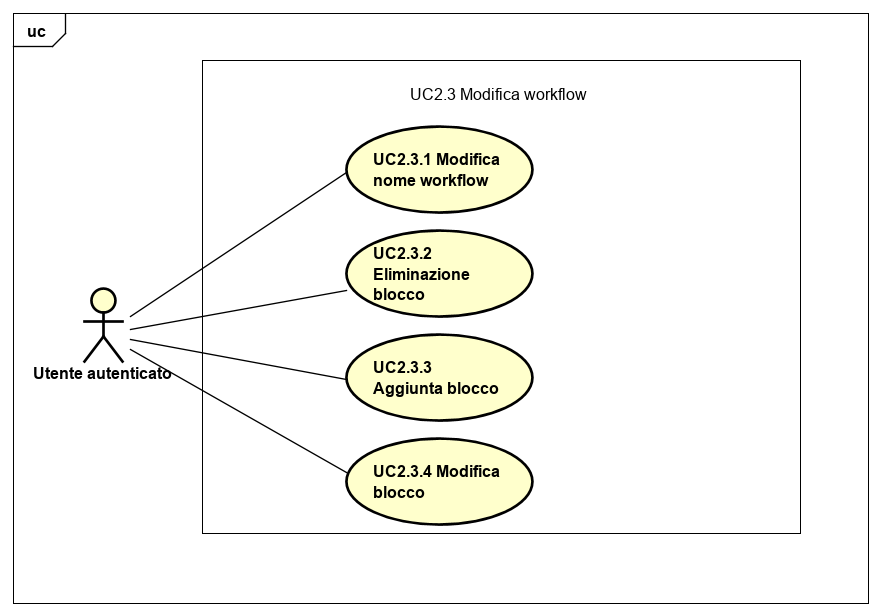
\includegraphics[scale=0.4]{./Diagram/UC2-3.png}
	\caption{Modifica workflow }\label{}
\end{figure}
\begin{itemize}
	\item \textbf{Attori primari}: Utente autenticato;
	\item \textbf{Descrizione:} L'attore modifica un \textit{workflow$_{G}$};
	\item \textbf{Precondizione:} Il sistema mette a disposizione un form per la modifica di un workflow;
	\item \textbf{Flusso principale degli eventi:}
	\begin{enumerate}
		\item L'attore può cambiare il nome del\glossario{workflow}(UC2.3.1);
		\item L'attore può eliminare un blocco dal workflow (UC2.3.2);
		\item L'attore può aggiungere un blocco nel workflow (UC2.3.3);
		\item L'attore può modificare la configurazione di un blocco presente nel workflow (UC2.3.4).
	\end{enumerate}
	\item \textbf{Postcondizione:} Il\glossario{workflow}è stato modificato.
\end{itemize}
\section{Caso d'uso UC2.3.1: Modifica nome workflow}
\begin{itemize}
	\item \textbf{Attori primari}: Utente autenticato;
	\item \textbf{Descrizione:} L'attore modifica il nome del \textit{workflow$_{G}$};
	\item \textbf{Precondizione:} Il sistema mette a disposizione un campo per l'inserimento del nuovo nome;
	\item \textbf{Flusso principale degli eventi:}
	\begin{enumerate}
		\item L'attore inserisce il nuovo nome del workflow.
	\end{enumerate}
	\item \textbf{Postcondizione:} Il form di creazione del workflow contiene il nuovo nome del workflow.
\end{itemize}
\section{Caso d'uso UC2.3.2: Eliminazione blocco }
\begin{itemize}
	\item \textbf{Attori primari}: Utente autenticato.
	\item \textbf{Descrizione:} L'attore rimuove il blocco che non desidera più dal \textit{workflow$_{G}$};
	\item \textbf{Precondizione:} Il sistema fornisce un comando per l'eliminazione del blocco;
	\item \textbf{Flusso principale degli eventi:}
	\begin{enumerate}
		\item L'attore elimina il blocco.
	\end{enumerate}
	\item \textbf{Postcondizione:} Il workflow non contiene più il blocco indesiderato dall'attore.
\end{itemize}
\section{Caso d'uso UC2.3.3: Aggiunta blocco }
\begin{itemize}
	\item \textbf{Attori primari}: Utente autenticato;
	\item \textbf{Descrizione:} L'attore aggiunge il nuovo blocco al \textit{workflow$_{G}$};
	\item \textbf{Precondizione:} Il sistema mette a disposizione un form per l'aggiunta del blocco;
	\item \textbf{Flusso principale degli eventi:}
	\begin{enumerate}
		\item L'attore aggiunge il blocco;
		\item L'attore configura il nuovo blocco.
	\end{enumerate}
	\item \textbf{Postcondizione:} Il workflow contiene il nuovo blocco configurato.
\end{itemize}
\section{Caso d'uso UC2.3.4: Modifica blocco }
\begin{itemize}
	\item \textbf{Attori primari}: Utente autenticato;
	\item \textbf{Descrizione:} L'attore modifica la configurazione del blocco che compone il \textit{workflow$_{G}$};
	\item \textbf{Precondizione:} Il sistema mette a disposizione un form per la modifica dei blocchi;
	\item \textbf{Flusso principale degli eventi:}
	\begin{enumerate}
		\item L'attore modifica la configurazione del blocco.
	\end{enumerate}
	\item \textbf{Postcondizione:} Il blocco desiderato dall'attore è stato riconfigurato.
\end{itemize}
\section{Caso d'uso UC2.4: Modifica account Amazon }
\begin{itemize}
	\item \textbf{Attori primari}: Utente autenticato;
	\item \textbf{Descrizione:} L'attore cambia il proprio account \textit{Amazon$_{G}$};
	\item \textbf{Precondizione:} Il sistema mette a disposizione un form per la modifica dell'account Amazon.
	\item \textbf{Flusso principale degli eventi:}
	\begin{enumerate}
		\item L'attore, attraverso il form di Amazon, sceglie il nuovo account.
	\end{enumerate}
	\item \textbf{Postcondizione:} Il sistema è collegato al nuovo account Amazon.
	\item \textbf{Estensione:}
	\begin{itemize}
		\item Visualizzazione dell'errore di cambio Account (UC2.4.1);
	\end{itemize}
\end{itemize}
\section{Caso d'uso UC2.4.1: Errore di cambio account Amazon }
\begin{itemize}
	\item \textbf{Attori primari}: Utente autenticato;
	\item \textbf{Descrizione:} L'attore ha inserito dei dati non corretti e non riesce a collegarsi al nuovo account \textit{Amazon$_{G}$};
	\item \textbf{Precondizione:} Il sistema non riesce a collegarsi all'account Amazon;
	\item \textbf{Flusso principale degli eventi:}
	\begin{enumerate}
		\item L'attore può inserire nuovamente i dati nel form di Amazon;
		\item L'attore può tornare al vecchio account Amazon.
	\end{enumerate}
	\item \textbf{Postcondizione:} Il sistema è correttamente collegato a un account Amazon.
\end{itemize}
\section{Caso d'uso UC2.5: Logout }
\begin{itemize}
	\item \textbf{Attori primari}: Utente autenticato;
	\item \textbf{Descrizione:} L'attore effettua il logout dall'applicazione;
	\item \textbf{Precondizione:} Il sistema fornisce un metodo per permettere all'utente di disconnettersi dal sistema;
	\item \textbf{Flusso principale degli eventi:}
	\begin{enumerate}
		\item L'attore si disconnette dal sistema.
	\end{enumerate}
	\item \textbf{Postcondizione:} Il sistema non riconosce più l'utente.
\end{itemize}

	\label{LastPage}

\end{document}